%! TEX root = paper.tex

\section{Approach}\label{sec:approach}

We propose two different approaches to address the relocalization proble. First, a local approache is based on the PTAM implementation, where two steps are performed. The first step has been named \textit{Place Finder} and the second \textit{Real Pose Recognition}. Multiple methods will be proposed to solve the second step. Then, on the other side, a global approach will be proposed. In this case machine learning methods (\textit{ferns}) will be used to recognize points in space.

\subsection{PTAM method}
\label{sub:ptam_method}

PTAM~\cite{KleinMurray2007} is a VO algorithm based on keyframes and so the relocalization method proposed is based on keyframes as well. Every keyframe is associated with a camera pose that will be used to relocalize. During the relocalization there are two steps involved. We called the first step \textit{Place Finder} and the second \textit{Real Pose Finder}.

\subsubsection{Place Finder}
\label{ssub:place_recognition}

During this step, the algorithm tries to find the keyframe image most similar to the last acquired image. The pose associated with the most similar keyframe is used as an initial rough estimation of the current pose. The similarity score should be invariant to small view point changes because the new acquired image will, most probably, never be taken from the same pose as any of the keyframes. Also it should be fast to compute.\\

The used similarity score is the Cross Correlation between images meaning the sum of the squared error between two zero-mean images as in~\ref{eq:CC}. To make to computation faster both images are resized become $40\times30$. Then, to make the images more resistant to view point changes it is blurred with a $3\times3$ Gaussian kernel with $\sigma=2.5$. The resulting image is a resized, blurred and zero-mean image called \textit{small-blurry-image}.\\

\begin{equation}
  d_{CC} = \sum_{x,y} [(I(x,y) - \bar{I}) - (G(x,y) - \bar{G})]^2
  \label{eq:CC}
\end{equation}


\subsubsection{ESM Real Pose Finder}
\label{ssub:real_pose_finder}

The second step of the PTAM relocalization algorithm found, in order to refine the pose of the most similar keyframe to explain the current pose of the camera. During this step, in the implementation from PTAM, only rotations are corrected. An image alignment through optimization algorithm (ESM~\cite{lovegrove2012parametric}) is used to find the $SE(2)$ transformation between the two, followed by a minimization to find a transformation in the world frame.\\

The Extended Second order Minimization algorithm (ESM)~\cite{lovegrove2012parametric} is based on the algorithm proposed by Lucas and Kanade \cite{Baker2004} in 1981. The goal of both algorithms is to align one template image $T$ to a different input image $I$ through a parametrised warping function. \\

With this goal an error function is defined on which the Gauss-Newton or Levenberg-Marquardt schemes can be applied. The error is the squared difference between the template image and the warped input image

\begin{equation}
  e = \sum_x [I(W(x;p)) - T(x)]^2
\end{equation}

The warping function is going to be in $SE(2)$, that is, translation and rotation of the image plane. The algorithm assumes that a current estimate of $p$ exists and iteratively tries improves it by increments $\Delta p$. On every  iteration equation~\ref{eq:delta_error} is solved on $\Delta p$ and then it is used to update $p$ as in eq.~\ref{eq:p_update}.\\

\begin{equation}
  \min_{\Delta p}  \sum_x [I(W(x;p + \Delta p)) - T(x)]^2
  \label{eq:delta_error}
\end{equation}

\begin{equation}
  p \leftarrow p + \Delta p
  \label{eq:p_update}
\end{equation}


The solution that minimizes eq.~\ref{eq:delta_error}  on $\Delta p$ can be found in a least squares sense. The equation needs to be derived and then set it equal to zero. 

The ESM algorithm used in PTAM is very similar to the derived above with the difference that while the Lucas-Kanade takes the gradient from the input image, ESM used both the gradient of the input image and the gradient of the template image and averages them.

\begin{equation}
  \nabla I = \frac{1}{2} \left[\nabla I_t + \nabla I_q \right]
\end{equation}

In Figure~\ref{fig:se3_error_1} the error of the overlapped images is visualized. It can be seen that translation and rotation are well corrected but there still is a misalignment caused mostly by a change on scale which is not taken into account during the alignment.\\


\begin{figure}[htpb]
  \centering
  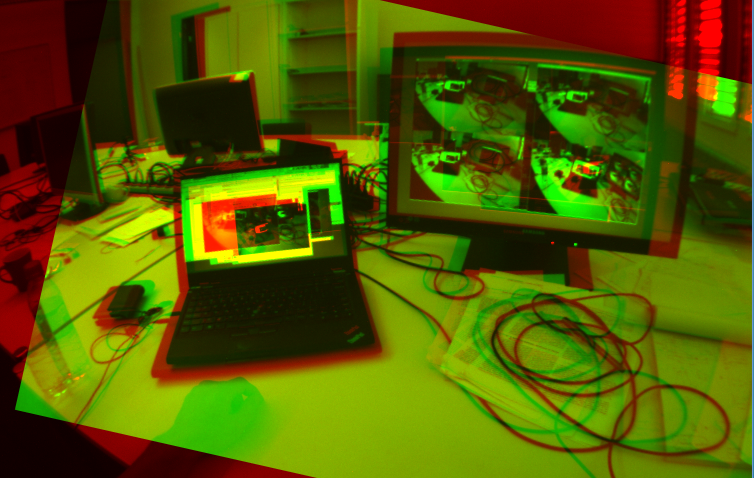
\includegraphics[width=8cm]{img/se2_error_1.png}
  \caption{$SE(2)$ transformation error visualization}
  \label{fig:se3_error_1}
\end{figure}


\subsubsection{Alternative Real Pose Finder}
\label{ssub:real_pose_finder_alternative}

During the mapping of an area, the VO algorithm finds landmarks in the world frame which are associated with detected featured points in keyframes (i.e. every featured point in an image is related to a $3D$ position in the world frame). Given a new image, some extracted featured points can be related to a keyframe using descriptor-matching which at the same time are related to world positions. From this information the full 6 DoF translation $SE(3)$ can be computed using the prospective three-point algorithm (P3P).\\

\begin{figure}[htpb]
  \centering
  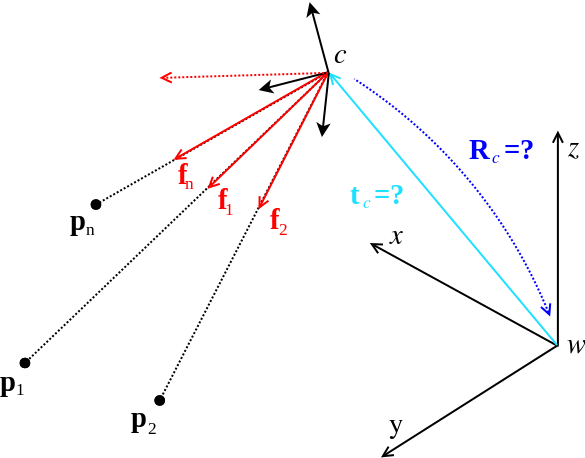
\includegraphics[width=0.6\linewidth]{img/absolute_central.png}
  \caption{From camera frame vectors $f$ (or image pixels if the camera calibration is available) and fix points $p$ the transformation between the two coordinate frames can be computed using the P3P algorithm. Image taken from \cite{kneipopengv}}
  \label{fig:img/absolute_centra}
\end{figure}

First, descriptors from every featured point are extracted. Second, a brute force KNN matching is performed from all the extracted descriptors from on image and all the descriptors of the second image. The first, and second most similar descriptor are retrieved. Then, only good matches are kept, that is, using the matching technique described by Lowe~\cite{lowe2004distinctive}, only matches with a descriptor ratio between the first and the second closest match of 0.8 or less are kept.\\

Finally, the three-point algorithm is fed with the pixel positions from the query image and the landmarks from the other. Because there are still outliers after the described simple filtering, this process is run in RANSAC~\cite{fischler1981random} framework. \\


Figures~\ref{fig:3pt_matches} is an example of the described above.\\

\begin{figure}[htpb]
  \centering
  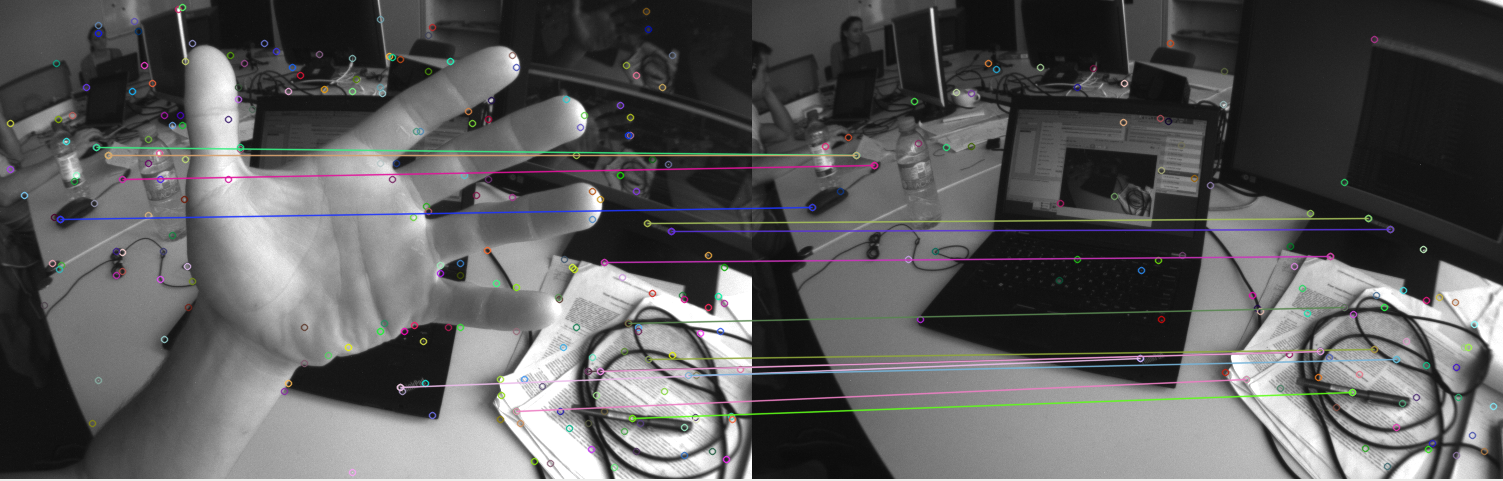
\includegraphics[width=1.0\linewidth]{img/3pt_matches_1.png}
  \caption{Accepted matches using SIFT}
  \label{fig:3pt_matches}
\end{figure}


\section{Using ferns}
\label{sec:using_ferns}

As said previously with the three-point algorithm it is possible to recover the 6 DoF of the camera pose from the relation from pixel coordinates and points in space. In this case machine learning techniques are used to model this relationship. In the classifier scheme, an object in space is a class and multiple views seen from the camera should all be classified as this class.\\

A \textit{fern}~\cite{Ozuysal2010} is a descriptor made from a set of binary tests such as in equation~\ref{eq:fern_test}. When used as a classifier, every possible evaluation of a \textit{fern} will contain a posterior probability distribution for every class.\\

\begin{equation}
  f_j =
  \left\{
    \begin{array}{l l}
      1, & \text{if} \quad I(d_j,1) < I(d_j,2) \\
      0, & \text{otherwise}
    \end{array} \right.
  \label{eq:fern_test}
\end{equation}


One \textit{fern} is usually not descriptive enough to correctly classify. In~\cite{Ozuysal2010} it is claimed that with 50 \textit{ferns} and $S=11$ a problem with 200 different classes is tractable. Regarding storage requirements, it would involve $50\times2^{11}\times200 = 20480000$ elements to be stored in memory. If these are stored as \textit{float} then 78 MB are needed, which is tractable. \\
